\documentclass{article}
\usepackage{fullpage}
\usepackage{nopageno} 
\usepackage{amsmath}
\usepackage{amssymb}
\usepackage{cancel}
\usepackage{tikz}
\usetikzlibrary{shapes.geometric, calc}
\allowdisplaybreaks

\newcommand{\abs}[1]{\left\lvert #1 \right\rvert}

\begin{document}
\title{Notes}
\date{April 28, 2014}
\maketitle
bijections

self-conjugate $\leftrightarrow$ distinct odd parts

odd-parts $\leftrightarrow$ distinct parts

\section*{homework}
prove that when you conjugate two partitions it reverses the majorization order.

induction on size of partition? notational question. give yourself some notation.

\[\lambda=\lambda_1+\lambda_2+\lambda_3+\dots+\lambda_k\]
\begin{align*}
  \mu\le\lambda\text{ so } \lambda_1+\dots+\lambda_i\ge\mu_1+\dots+\mu_i\\
  \mu=\mu_1+\mu_2+\dots+\mu_k
\end{align*}
\section*{schr\"{o}der paths: 8.5}
\subsubsection*{definition}
a dissection of a polygon is a partition of its interior into regions by inserting noncrossing diagonals.
  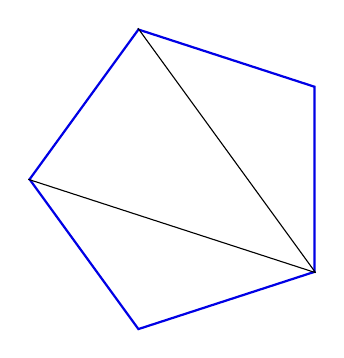
\begin{tikzpicture}
    \node (pol) [draw, thick, blue!90!black,rotate=90,minimum size=4cm,regular polygon, regular polygon sides=5] at (0,0) {}; 
    %\foreach \n [count=\nu from 1, remember=\n as \lastn, evaluate={\nu+\lastn}] in {1,2,...,4} 
    %\node[anchor=\n*(360/5)]at(pol.side \n){$a_{\nu}$};
    \draw (pol.corner 1) -- (pol.corner 3);
    \draw (pol.corner 3) -- (pol.corner 5);
    %\node[anchor=5*(360/5)]at(pol.side 5){$((a_1 a_2)(a_3 a_4))$};
  \end{tikzpicture}

question: how many dissections of triangle, square, pentagon? 1,3,11

question apply multiplication scheme like map to dissections to obtain bracketings

\subsubsection*{definition}
a bracketing of $a_1\dots a_n$ is a multiplication scheme where parentheses can enclose any  number of variables
\subsection*{theorem}
bracketings of n variables are in bijections with dissections of an $n+1$-gon.
\subsubsection*{definition}
a large schr\"{o}der path is a path  from $(0,0)$ to $(2n,0)$ with steps in the set which never go below the x-axis. note that dyck paths are schr\"{o}der paths with no $(1,0)$ steps

question how many large schr\"{o}der pths are there for n=1,2,3...
$R_n=2S_{n+1}$ where $R_n$ is large and $S_n$ is small.

question: what is a recurrance for $R_n$?

$R_n$ start with (0)+start with (1). $R_n=R_{n+1}+\sum\limits_{k=1}^n{R_{k-1}R_{n-k}}$. define $R_0=1$.
\end{document}
